Пусть теперь, как в исходной постановке задачи, параметр $\theta$ неизвестен. Тогда для реализуемости закона управления (\ref{control}) заменим величину $\theta$ на ее оценку $\hat{\theta}$:

\begin{equation}
    u = - \hat{\theta} x - \lambda x + \lambda g
\end{equation}

Если оценка $\hat{\theta}$ такая что, $\dot{\hat{\theta}} = - \gamma x \varepsilon$, где $\gamma$ - коэффициентом адаптации, то по методу функций Ляпунова можно показать, что целевое равенство (\ref{goal}) будет выполнено.

Проведем моделирование полученной замкнутой системы при различных значениях параметра $\gamma$, получим следующие графики:

\begin{figure}
    \centerline{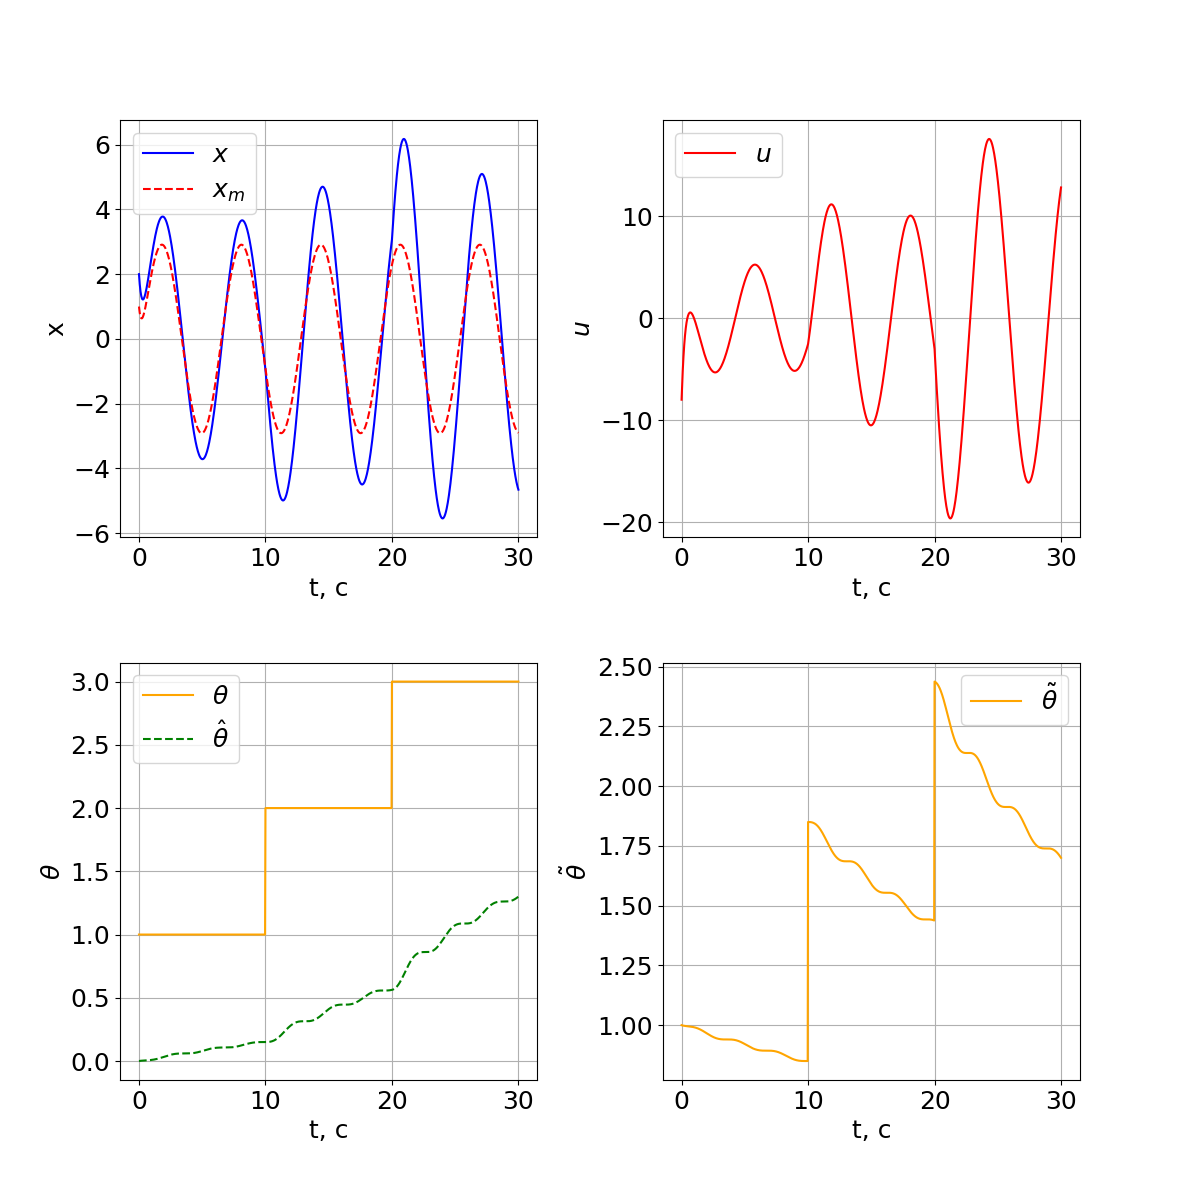
\includegraphics[width=\linewidth]{images/task_2_0.01.png}}
    \caption{График переходного процесса и управляющего воздействия, а также графика параметра $\theta$ и его оценки $\hat{\theta}$ для адаптивной системы с параметром $\gamma = 0.01$}
    \label{21}
\end{figure}

Как можно видеть, при маленьком коэффициенте адаптации, система не успевает дать правильную оценку параметру, так как изменение реального параметра происходит быстрее. Но при этом, целевое равенство (\ref{goal}) выполняется.

Рассмотрим результаты моделирования при других параметров $\gamma$:

\begin{figure}
    \centerline{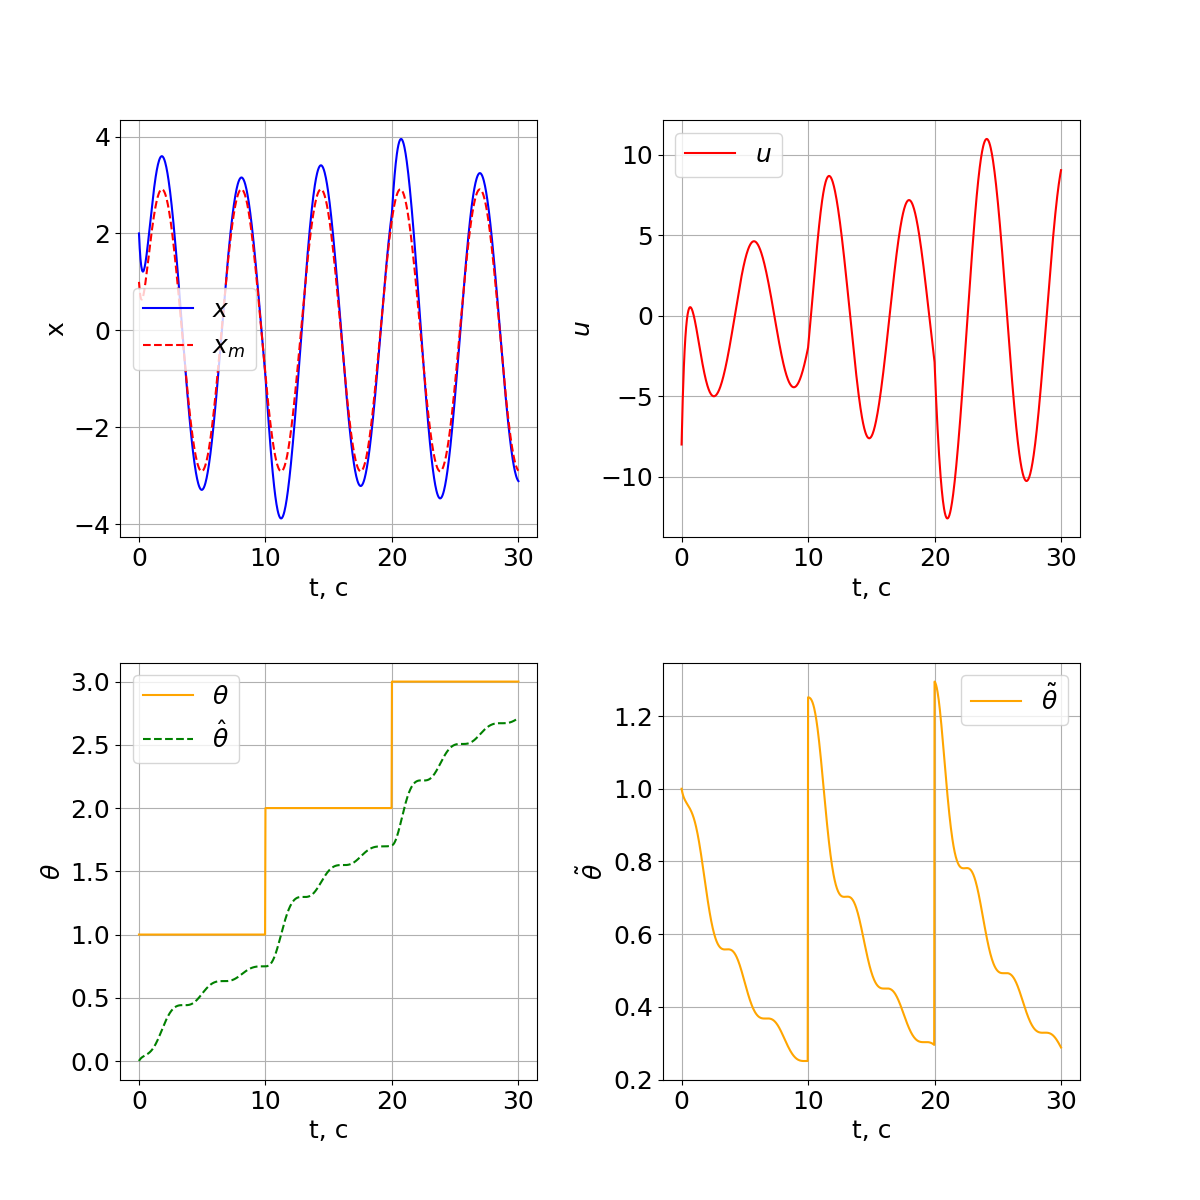
\includegraphics[width=\linewidth]{images/task_2_0.1.png}}
    \caption{График переходного процесса и управляющего воздействия, а также графика параметра $\theta$ и его оценки $\hat{\theta}$ для адаптивной системы с параметром $\gamma = 0.1$}
    \label{22}
\end{figure}

\begin{figure}
    \centerline{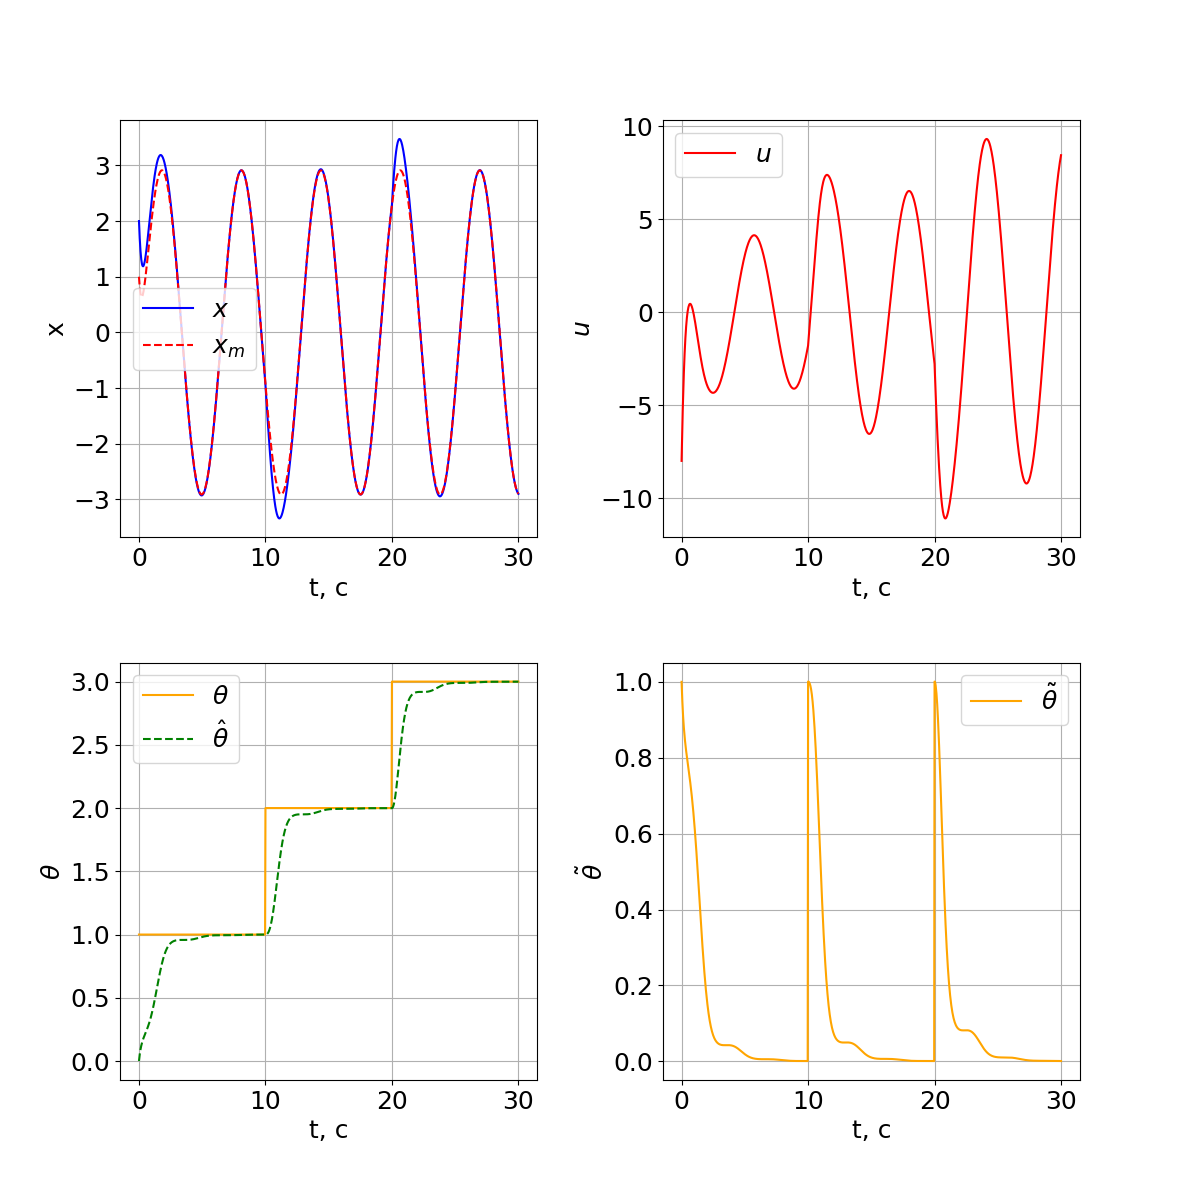
\includegraphics[width=\linewidth]{images/task_2_0.5.png}}
    \caption{График переходного процесса и управляющего воздействия, а также графика параметра $\theta$ и его оценки $\hat{\theta}$ для адаптивной системы с параметром $\gamma = 0.5$}
    \label{23}
\end{figure}

\begin{figure}
    \centerline{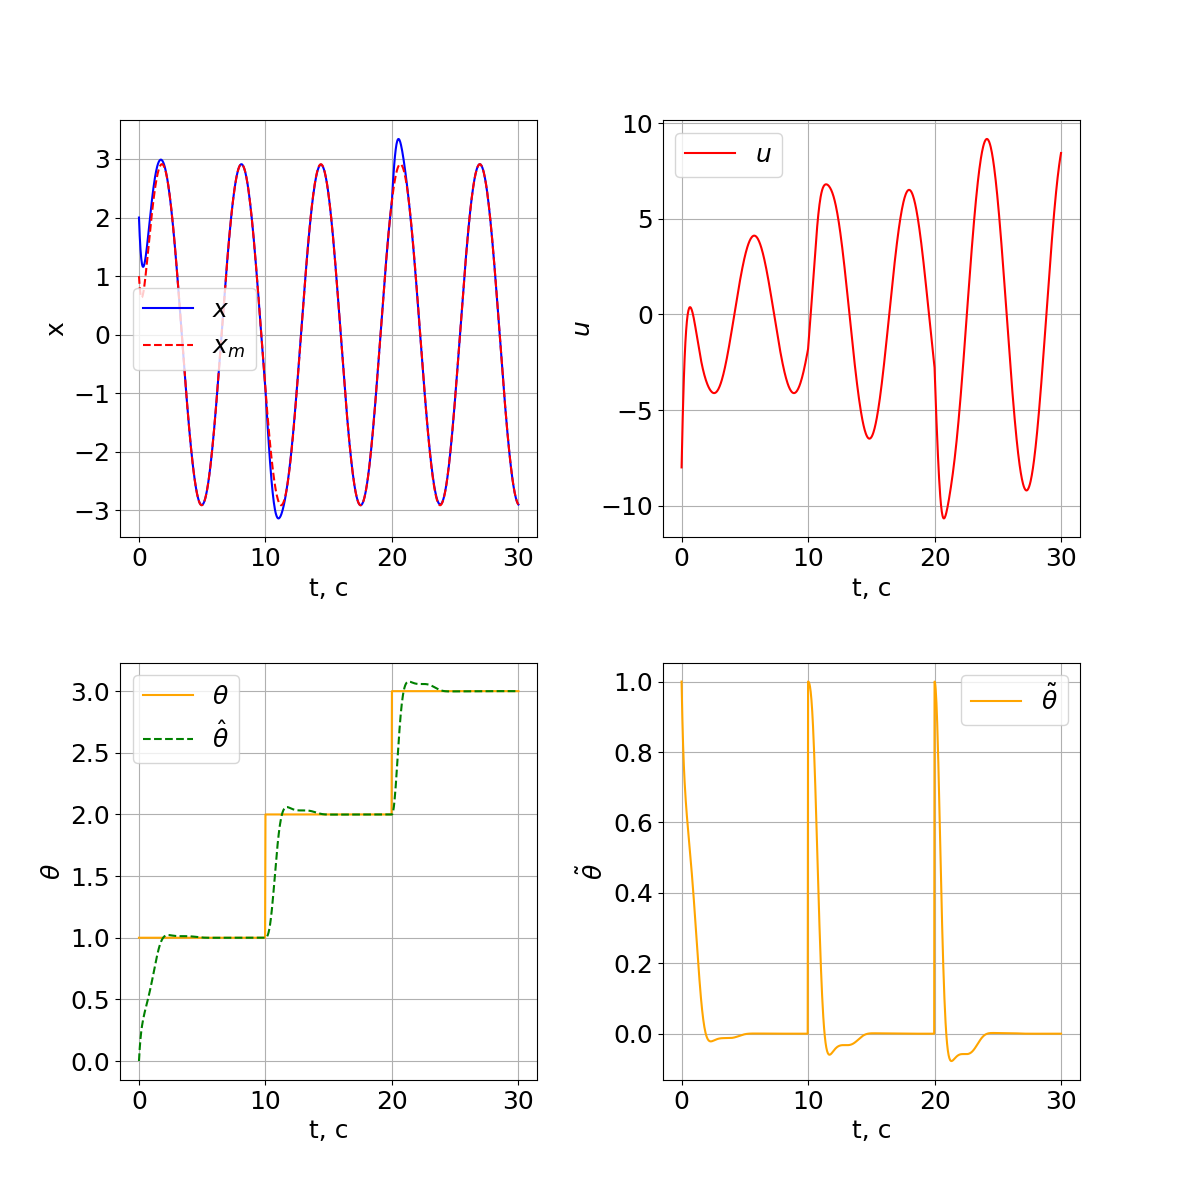
\includegraphics[width=\linewidth]{images/task_2_1.0.png}}
    \caption{График переходного процесса и управляющего воздействия, а также графика параметра $\theta$ и его оценки $\hat{\theta}$ для адаптивной системы с параметром $\gamma = 1.0$}
    \label{24}
\end{figure}

\begin{figure}
    \centerline{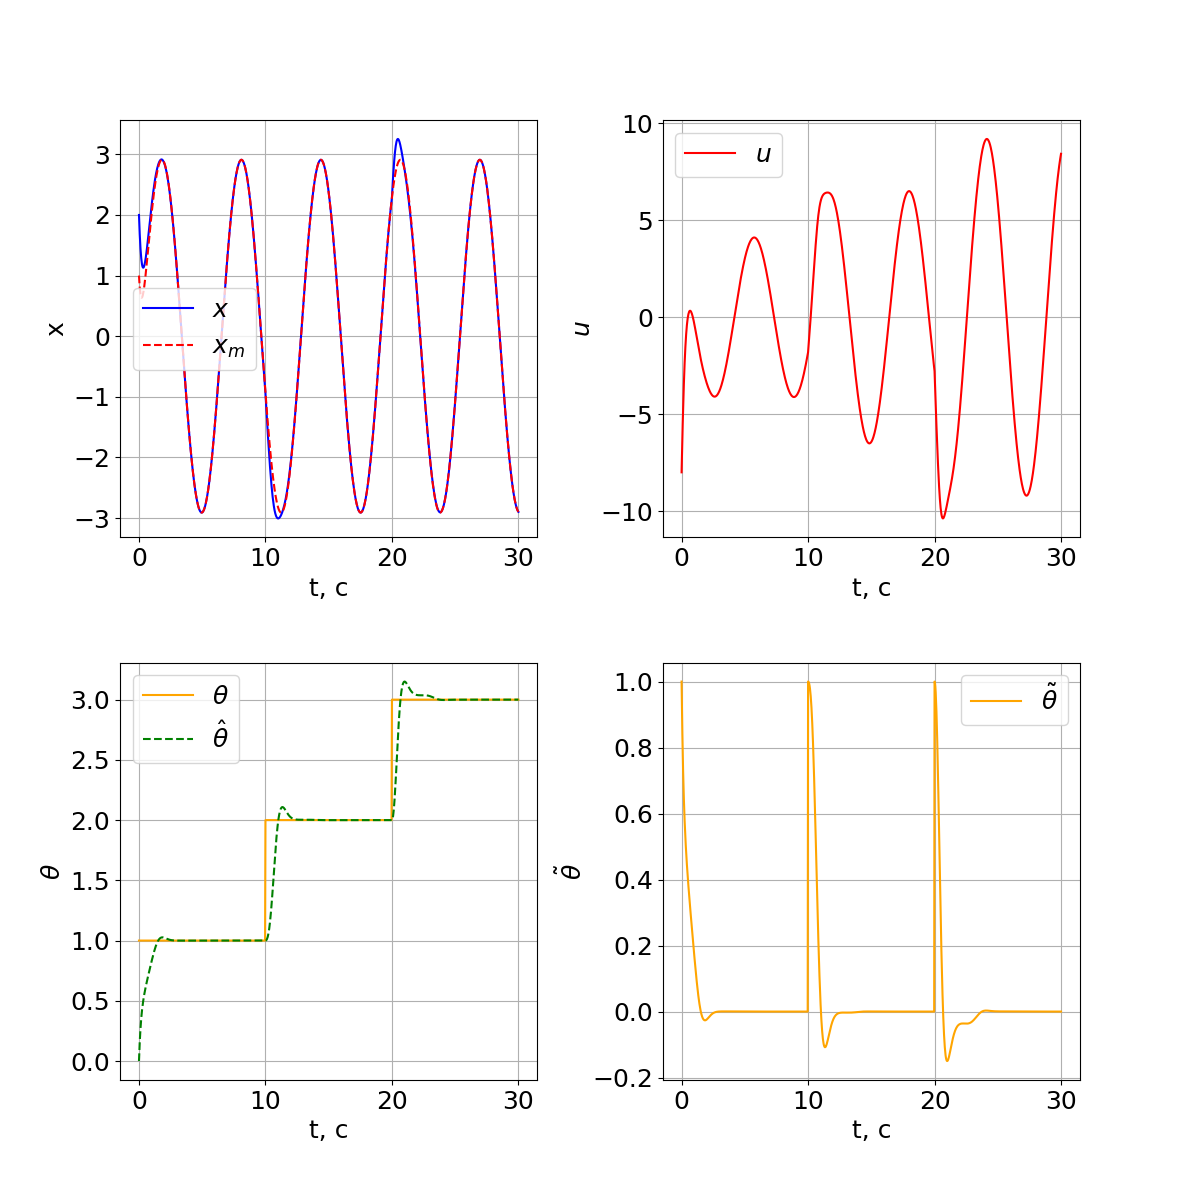
\includegraphics[width=\linewidth]{images/task_2_1.5.png}}
    \caption{График переходного процесса и управляющего воздействия, а также графика параметра $\theta$ и его оценки $\hat{\theta}$ для адаптивной системы с параметром $\gamma = 1.5$}
    \label{25}
\end{figure}

Можно заметить, что чем больше параметр $\gamma$, тем быстрее алгоритм адаптации сводит ошибку $\tilde{\theta}$ к нулю, и значит тем быстрее система адаптируются к скачкообразным изменениям параметра $\theta$.